\documentclass[tikz,border=6pt]{standalone}
\usepackage{amsmath,amssymb}
\usetikzlibrary{arrows.meta}

\newcommand{\IT}{\mathbb{T}}
\newcommand{\IL}{\mathbb{L}}

\begin{document}
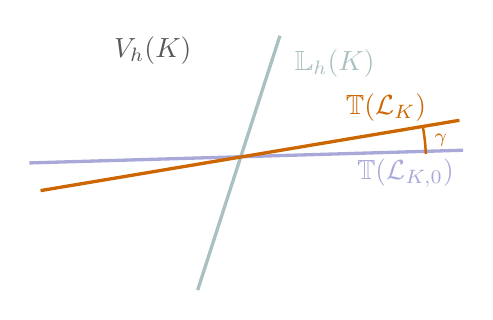
\begin{tikzpicture}[scale=0.95,>=Latex]

% colors
\colorlet{cTT}{blue!22}
\colorlet{cTL}{teal!22}
\colorlet{cZero}{black!4}

% lifting space IL_h(K), slightly tilted
\draw[very thick,cTL!85!black] (-0.55,-1.75) -- (0.55,1.65);
\node[anchor=west,text=cTL!85!black] at (0.62,1.28) {$\IL_h(K)$};

% prototype Trefftz space
\draw[very thick,cTT!85!black] (-2.8,-0.05) -- (3.0,0.12);
\node[anchor=west,text=cTT!85!black] at (1.45,-0.18)
  {$\IT(\mathcal L_{K,0})$};

% perturbed Trefftz space
\draw[very thick,orange!80!black] (-2.65,-0.42) -- (2.95,0.52);
\node[anchor=west,text=orange!80!black] at (1.3,0.69)
  {$\IT(\mathcal L_K)$};

% tiny angle marker between the two Trefftz spaces
\draw[orange!80!black, line width=0.9pt]
  (2.5,0.07) arc[start angle=2,end angle=10,radius=2.5];
\node[text=orange!80!black, font=\scriptsize] at (2.7,0.25) {$\gamma$};

% ambient space
\node[text=black!65] at (-1.15,1.45)
  {$V_h(K)$};

\end{tikzpicture}
\end{document}
